\documentclass[notitlepage,a4paper,twoside,10pt]{article}

\usepackage{mathpazo} 
\usepackage{ngerman} 
\usepackage[latin1]{inputenc} 
\usepackage[T1]{fontenc} 
\usepackage[pdftex]{graphicx} 
\usepackage[pdftex,bookmarks=true,colorlinks,linkcolor=blue,urlcolor=blue,citecolor=blue]{hyperref} 

%opening
\title{E-Mail jenseits der �berwachung}
\author{Unix / Linux}
\date{\today}

\hypersetup {
    pdftitle= {E-Mail jenseits der �berwachung}
    pdfkeywords= {anonyme E-Mail AnonBox Susimail Verschl�sselung GnuPG Quicksilver Mixmaster Internet Anonymit�t }
}


\begin{document}
\maketitle
\begin{abstract}
Auch bei der Nutzung von GnuPG oder S/MIME f�r die Verschl�sselung von E-Mails ist es mitlesenden Dritten m�glich, Absender und Empf�nger zu protokollieren und anhand der erfassten Daten Kommunikationsprofile zu erstellen. Insbesondere die Vorratsdatenspeicherung und die darauf aufbauenden internationalen ESTI-Standards f�r Geheimdienste und Strafverfolger zeigen, dass diese nicht verschl�sselbaren Informationen f�r die �berwachung bedeutsam sind.\\

Es gibt mehrere Projekte, die einen �berwachungsfreien Austausch von Nachrichten erm�glichen und somit beispielsweise f�r investigative Journalisten und deren Informanten den n�tigen Schutz bieten und die Erstellung von Kommunikationsprofilen f�r E-Mails behindern.
\end{abstract}

\section{Anonyme E-Mail Accounts}
Im Kapitel Anonymisierungsdienste gibt es Anleitungen, wie man mit JonDo \& Thunderbird oder mit Tor \& Thunderbird einen anonymen E-Mail Account nutzen k�nnte. Als E-Mail Provider kann man einen zuverl�ssigen Anbieter im Web nehmen. Au�erdem bieten I2P und Tor spezielle L�sungen: 
\begin{itemize}
 \item Das Invisible Internet Project (I2P) bietet mit Susimail einen anonymen Mailservice inclusive SMTP- und POP3-Zugang und Gateway ins Web oder mit I2P Bote einen serverlosen, verschl�sselten Maildienst. 
 \item TorMail gibt es als Hidden Service unter http://jhiwjjlqpyawmpjx.onion mit POP3 und SMTP Service und ist auch aus dem Web unter xxx@tormail.net erreichbar.
 \item Tor Privat Messaging unter http://4eiruntyxxbgfv7o.onion/pm/ ist ein Tor Hidden Service im Onionland, um Textnachrichten unbeobachtet auszutauschen. Der Dienst kann nur im Webinterface genutzt werden.
\end{itemize}

\textbf{Hinweis:} Informationen �ber Langzeitkommunikation k�nnen ein Pseudonym deanonymisieren. Anhand der Freunde in der E-Mail Kommunikation sind Schlussfolgerungen auf ihre reale Identit�t m�glich. Wenn sie einen wirklich anonymen E-Mail Account f�r eine bestimmte Aufgabe ben�tigen - z.B. f�r Whistleblowing - dann m�ssen sie einen neuen Account erstellen. L�schen sie den Account, sobald sie ihn nicht mehr brauchen.

\section{Private Messages in Foren nutzen}
Viele Diskussionsforen im Internet bieten die M�glichkeit, private Nachrichten zwischen den Mitgliedern zu verschicken. Die Nachrichten werden in der Datenbank des Forums gespeichert und nicht per E-Mail durch das Netz geschickt.\\

Eine b�se Gruppe ganz gemeiner Terroristen k�nnte sich also in einem Forum anmelden, dessen Diskussionen sie �berhaupt nicht interessieren. Dort tauschen sie die Nachrichten per PM (Private Message) aus und keiner bemerkt die Kommunikation. Es ist vorteilhaft, wenn das Forum komplett via HTTPS nutzbar ist und nicht beim Login HTTPS anbietet.\\

Die Nachrichten kann man mit OpenPGP verschl�sseln, damit der Admin des Forums nichts mitlesen kann. Die Verwendung von Anonymisierungsdiensten sichert die Anonymit�t.

\section{alt.anonymous.messages}
Um die Zuordnung von Absender und Empf�nger zu erschweren, kann man das Usenet nutzen. In der Newsgruppe \textit{alt.anonymous.messages} werden st�ndig viele Nachrichten gepostet und sie hat tausende Leser. Jeder Leser erkennt die f�r ihn bestimmten Nachrichten selbst. Es ist eine Art schwarzes Brett.\\

Es ist sinnvoll, die geposteten Nachrichten zu verschl�sseln. Daf�r sollte der Empf�nger einen OpenPGP-Key bereitstellen, der keine Informationen �ber seine Identit�t bietet. Normalerweise enth�lt ein OpnePGP-Schl�ssel die E-Mail Adresse des Inhabers. Verwendet man einen solchen Schl�ssel ist der Empf�nger nat�rlich deanomynisiert.\\

Au�erdem sollte man seine Antworten nicht direkt als Antwort auf ein Posting ver�ffentlichen. Da der Absender in der Regel bekannt ist (falls keine Remailer genutzt wurden) kann aus den Absendern eines zusammengeh�renden Thread ein Zusammenhang der Kommunikationspartner ermittelt werden.


\section{Mixmaster Remailer}
Der Versand einer E-Mail �ber Remailer-Kaskaden ist mit der Versendung eines Briefes vergleichbar, der in mehreren Umschl�gen steckt. Jeder Empf�nger innerhalb der Kaskade �ffnet einen Umschlag und sendet den darin enthaltenen Brief ohne Hinweise auf den vorherigen Absender weiter. Der letzte Remailer der Kaskade liefert den Brief an den Empf�nger aus.\\

\begin{figure}[htb]
\begin{center}
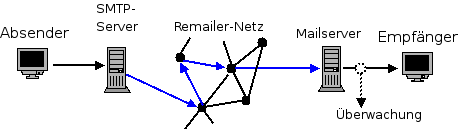
\includegraphics[scale=0.55]{../grafiken/remailer_mm.png}
\caption{Konzept einer anonymen E-Mail}
\label{abb:remailer}
\end{center}
\end{figure}

Technisch realisiert wird dieses Prinzip mittels asymmetrischer Verschl�sselung. Der Absender w�hlt aus der Liste der verf�gbaren weltweit verteilten Remailer verschiedene Server aus, verschl�sselt die E-Mail mehrfach mit den �ffentlichen Schl�sseln der Remailer in der Reihenfolge ihres Durchlaufes und sendet das Ergebnis an den ersten Rechner der Kaskade. Dieser entschl�sselt mit seinem geheimen Schl�ssel den ersten Umschlag, entnimmt dem Ergebnis die Adresse des folgenden Rechners und sendet die jetzt (n-1)-fach verschl�sselte E-Mail an diesen Rechner. Der letzte Rechner der Kaskade liefert die E-Mail an den Empf�nger aus.\\

Mitlesende Dritte k�nnen lediglich protokollieren, dass der Empf�nger eine E-Mail unbekannter Herkunft und evtl. unbekannten Inhaltes (verschl�sselt mit OpenPGP oder S/MIME) erhalten hat. Es ist ebenfalls m�glich, Beitr�ge f�r News-Groups anonym zu posten.\\

Um die Traffic-Analyse zu erschweren, wird die Weiterleitung jeder E-Mail innerhalb der Kaskade verz�gert. Es kann somit 2\dots12h dauern, ehe die Mail dem Empf�nger zugestellt wird! Sollte der letzte Remailer der Kette die Nachricht nicht zustellen k�nnen (z.B. aufgrund eines Schreibfehlers in der Adresse), erh�lt der Absender keine Fehlermeldung. Der Absender ist ja nicht bekannt.\\

\textbf{Wichtig:} Bei gro�en E-Mail Providern werden die anonymen E-Mails aus dem Mixmaster Netzwerk h�ufig als Spam einsortiert. Es ist somit nicht sichergestellt, dass der Empf�nger die Mail wirklich zur Kenntnis nimmt! Oft beschweren sich Nutzer bei mir, das ihre Testmails an den eigenen Account nicht ankommen, weil sie auch nicht in den Spam-Ordner schauen. 

\textbf{Wichtig:} Da die E-Mail keine Angaben �ber den Absender enth�lt, funktioniert der \textit{Antworten-Button} der Clients auf der Empf�ngerseite nicht! Die Antwort-Mail geht dann an den letzten Remailer der Kette, der sie in die Tonne wirft. Der Text der E-Mail sollte einen entsprechenden Hinweis enthalten!\\

Software zur Versendung anonymer E-Mails via Mixmaster:
\begin{itemize}
 \item F�r Windows gibt es \textit{Quicksilver} \href{https://quicksilvermail.net}{https://quicksilvermail.net}
 \item F�r Linux gibt es \textit{mixmaster}. Das Paket ist in allen Distributionen enthalten.
 \item Wer sich nicht mit der komplizierten Konfiguration besch�ftigen m�chte, der kann eine Live-CD nutzen. Die JonDo Live-CD enth�lt \textit{mixmaster}. Eine Anleitung zum Sender einer anonymen E-Mail findet man in der Online-Hilfe zur Live-CD.
\end{itemize}

\section{Mixmaster f�r Unix/Linux}

\subsection{Mixmaster installieren (Source)}
Die Sourcen von Mixmaster stehen unter \href{http://mixmaster.sourceforge.net}{http://mixmaster.sourceforge.net} zum Download bereit. F�r die �bersetzung werden die Entwicklerpakete folgender Komponenten ben�tigt, welche von nahezu allen Distributionen bereitgestellt werden:
 
\begin{itemize}
\item vi Editor
\item ncurses Bibliothek
\item OpenSSL Bibliothek
\item PCRE Bibliothek
\item zlib Bibliothek
\item OpenPGP Programm (z.B. GnuPG)
\end{itemize} 
 
Nach dem Download ist das Archiv zu entpacken und in das neu angelegte Verzeichnis zu wechseln. Hier ist das Kommando \textit{./Install} einzugeben.\\

Die Installationsroutine stellt einige kurze Fragen und bietet sinnvolle Vorgaben. Als Installationsverzeichnis ist es sinnvoll \textit{\$HOME/.Mix} zu �bernehmen. Die Frage \textit{Do you want to set up a remailer?} ist mit ENTER zu verneinen.\\

Die Meldung \textit{Client installation complete.} zeigt den erfolgreichen Abschluss der Installation an.\\

Im Anschlu� k�nnen die Remailer Listen initialisiert werden. Diese Listen enthalten die ben�tigten Informationen �ber nutzbare Remailer, die unterst�tzten Features und die �ffentlichen Schl�ssel der Remailer und sollten bei der Versendung einer E-Mail nicht �lter als 24h sein.
\begin{verbatim}
   > ~/.Mix/mixmaster --update-pinger-list
   > ~/.Mix/mixmaster --update-stats=noreply
\end{verbatim}

Sollte der Server \textit{noreply} nicht erreichbar sein, k�nnen \textit{deuxpi} oder andere Pinger  genutzt werden. Eine vollst�ndige �bersicht �ber alle Mixmaster-Pinger bietet \href{http://www.noreply.org}{http://www.noreply.org}. Zuk�nftige Updates der Listen k�nnen dem Daemon \textit{mixmaster-smtp} �berlassen werden.

\subsection{Mixmaster-SMTP installieren}
\textit{mixmaster-smtp} ist ein kleines Perl-Script, welches einen SMTP-Server bereitstellt, der von beliebigen E-Mail Clients versendete Mails an Mixmaster zur anonymen Versendung weiterleitet. Au�erdem �bernimmt es das Update der Remailer Listen bei Notwendigkeit.\\

Die \textbf{Sourcen} stehen unter \href{https://www.awxcnx.de/wabbel.htm}{https://www.awxcnx.de/wabbel.htm} zum Download bereit. Nach dem Entpacken des Archives k�nnte man das Script und die Manualpage mit \textit{./Install} nach /usr/local/bin bzw. /usr/local/man/man1 kopieren. Dieser Schritt ist aber nicht zwingend n�tig. Das Script im Unterverzeichnis \textit{bin/} startet aus beliebigen Verzeichnissen.\\

Das Script ben�tigt einige Perl Module f�r die Arbeit. Diese k�nnen als User \textit{root} via CPAN installiert werden:
\begin{verbatim}
   # perl -MCPAN -e shell
\end{verbatim} 

Nachdem die Fragen zur Initialiserung des CPAN-Moduls beantwortet wurden, sind am CPAN-Prompt folgende Kommandos einzugeben:
\begin{verbatim}
   cpan> install Net::Server::Daemonize
   cpan> install Net::Server::Mail::ESMTP
   cpan> exit
\end{verbatim}

Im Anschluss sollte das Script \textit{mixmaster-smtp} problemlos starten. Die n�tig Konfiguration wird in der Regel korrekt erkannt. Kleine Apassungen sind weiter unten beschrieben.\\

Das Archiv enth�lt im Verzeichnis \textit{init.d} drei Startscripte (f�r Debian/Ubuntu, Gentoo und SuSE), um den Daemon beim Booten automatisch zu starten. Diese werden wie folgt installiert:
\begin{itemize}
 \item Debian / Ubuntu
\begin{verbatim}
# cp init.d/mixmaster-smtp.debian /etc/init.d/mixmaster-smtp
# update-rc.d mixmaster-smtp defaults
\end{verbatim} 
\item SuSE Linux
\begin{verbatim}
# cp init.d/mixmaster-smtp.suse /etc/init.d/mixmaster-smtp
# insserv mixmaster-smtp
\end{verbatim} 
\end{itemize}

\subsection{Mixmaster konfigurieren}
Die Konfiguration erfolgt in der Textdatei \textit{\$HOME/.Mix/mix.cfg} oder global f�r alle User in der Datei \textit{/etc/mixmaster/client.conf}. Linux wird an dieser Stelle seinem Ruf als Volltext-Adventure gerecht.\\

F�r die Versendung an den ersten Remailer der Kaskade wird ein Name f�r den Absender und eine Absenderadresse ben�tigt. Es sind folgende Zeilen in der Konfiguration hinzuzuf�gen:\\

\begin{tabular}{ll}
NAME  & realer Name \\ 
ADDRESS  &  reale E-Mail Adresse\\ 
\end{tabular} \\

Mixmaster sollte f�r die Versendung der anonymen E-Mails an den ersten Remailer der Kaskade m�glichst den lokalen Mail Transfer Agenten nutzen, um eine �berfl�ssige Protokollierung durch den Mailserver des Providers zu vermeiden. Wenn \textit{sendmail} funktioniert, ist folgende Vorgabe korrekt:\\

\begin{tabular}{ll}
SENDMAIL &  sendmail -t\\
\end{tabular} \\

Soll statt dessen ein lokaler oder externer SMTP-Server f�r die Versendung genutzt werden, ist statt SENDMAIL folgende Zeile hinzuzuf�gen:\\

\begin{tabular}{ll}
SMTPRELAY &  mail.server.tld\\
\end{tabular} \\

Erfordert der SMTP-Server eine Anmeldung via SMTP-Auth, sind folgende Zeilen in der Konfigurationsdatei hinzuzuf�gen:\\

\begin{tabular}{ll}
SMTPUSERNAME & SMTP-UserName\\
SMTPPASSWORD & SMTP-Passwort\\
\end{tabular} \\

Ausserdem sind in der Konfiguration die Schl�sselringe f�r OpenPGP-Verschl�sselung anzugegeben. Verwendet man GnuPG, sind folgende Zeilen korrekt:\\

\begin{tabular}{ll}
PGPPUBRING & /home/<username>/.gnupg/pubring.gpg\\
PGPSECRING & /home/<username>/.gnupg/secring.gpg\\
\end{tabular} \\


\subsection{Mixmaster-SMTP konfigurieren}
Mixmaster-SMTP nutzt die Konfigurationsdatei \textit{\$HOME/.Mix/smtp.conf} oder global f�r alle User in der Datei \textit{/etc/mixmaster/smtp.conf}. Ein Beispiel ist im Verzeichnis \textit{conf} des Quellpaketes enthalten.\\

Wer eine �ltere Version von mixmaster vor 3.0rc1 nutzt, muss das Update der Remailer Statistiken in der Konfiguration deaktivieren und sich selbst drum k�mmern:\\

\begin{tabular}{ll}
REMAILER\_UPDATE & no\\
\end{tabular} \\

Das von P. Palfrader betreute Mixmaster-Paket f�r Debian GNU/Linux enth�lt ein eigenes Script f�r das Update. Wer dieses Paket nutzt, sollte das Update entsprechend konfigurieren:\\

\begin{tabular}{ll}
REMAILER\_UPDATE & debian\\
\end{tabular} \\

Wer die Software f�r den Onion Router (Tor) installiert hat, kann dieses Netzwerk nutzen, um keine Spuren in den Logs des Providers zu hinterlassen:\\

\begin{tabular}{ll}
TORIFY\_UPDATES & yes\\
\end{tabular} \\

\subsection{Installation f�r Debian GNU/Linux}
Debian GNU/Linux und Ubuntu enthalten ein fertiges \textit{mixmaster}-Paket. F�r \textit{mixmaster-smtp} gibt es ein Packet im Wabbel-Repository.  Die Einbindung des Wabbel-Repository ist auf der Website \href{https://www.awxcnx.de/wabbel.htm}{https://www.awxcnx.de/wabbel.htm} beschrieben.\\

 Anschlie�end sp�len die folgenden Kommandos alles n�tige auf die Platte und starten den Daemon \textit{mixmaster-smtp}
\begin{verbatim}
  # apt-get update && aptitude install mixmaster mixmaster-smtp
\end{verbatim}

Alle Pakete sind sinnvoll konfiguriert. Lediglich die Identit�t f�r die Versendung einer E-Mail an den ersten Remailer der Kaskade ist in \textit{/etc/mixmaster/client.conf} zu konfigurieren:\\

\begin{tabular}{ll}
NAME  & realer Name \\ 
ADDRESS  &  reale E-Mail Adresse\\ 
\end{tabular} \\

Sollte der Provider die Versendung von E-Mails von lokalen Rechnern unterbinden (Spamschutz), ist ein SMTPRELAY wie oben beschrieben, in der Datei \textit{/etc/mixmaster/client.conf} zu konfigurieren.

\subsection{Anonyme E-Mails mit Mixmaster versenden}
Wer mit dem \textbf{Editor vi} vertraut ist, kann Mixmaster auf der Kommandozeile starten, mit dem integrierten Editor eine E-Mail schreiben und anonym versenden.\\

\textbf{mixmaster-smtp} bietet die M�glichkeit, eine E-Mail mit dem bevorzugten E-Mail Client zu schreiben, zu verschl�sseln und zur anonymen Versendung an Mixmaster zu �bergeben. Auch das Update der Remailer Statistiken �bernimmt das Script bei Bedarf. Das folgende Kommando in einer Konsole(!) startet den Daemon etwas geschw�tzig, wenn er nicht beim Booten gestartet wurde:
\begin{verbatim}
   > mixmaster-smtp --verbose
\end{verbatim} 

Evtl. ist der vollst�ndige Pfad zum Script anzugeben. Es startet ein SMTP-Server, welcher unter der Adresse \textit{localhost:8025} auf E-Mails wartet. Im E-Mail Client ist ein weiterer SMTP-Server f�r den Versand zu konfigurieren und evtl. eine Identit�t anzulegen.\\

Eine dritte M�glichkeit nutzt einen beliebigen \textbf{Texteditor} oder besser eine komplette Textverarbeitung mit Rechtschreibpr�fung und Vorlagenverwaltung, um die E-Mail auf Basis der folgenden Vorlage zu schreiben, als TXT-Datei zu speichern und diese mit Mixmaster anonym zu versenden.
\begin{verbatim}
To:
Subject:
Mime-Version: 1.0
Content-Type: text/plain; charset=''utf-8''
Content-Transfer-Encoding: 8bit

Hallo alle miteinander,
hier beginnt der Inhalt
\end{verbatim} 

In den ersten beiden Zeilen ist die E-Mail-Adresse des Empf�ngers und der Betreff der Nachricht einzutragen.  Zwischen dem Header und dem eigentlichen Inhalt ist eine Leerzeile frei zu lassen.\\

Nachdem die Nachricht geschrieben wurde, ist die Datei unter einem neuen Namen als TXT-Datei zu speichern, beispielsweise unter
\textit{\$HOME/anon-email.eml}.\\

Diese E-Mail kann mit den folgenden Befehlszeilen versendet werden, welche f�r h�ufige Nutzung auch als Shell-Script gespeichert werden k�nnen:
\begin{verbatim}
  > ~/.Mix/mixmaster --update-stats=deuxpi
  > ~/.Mix/mixmaster -m ~/anon-email.eml
  > ~/.Mix/mixmaster -S
  > shred -u ~/anon-email.eml}
\end{verbatim} 

Der erste Befehl aktualisiert die Remailer-Statistiken und kann entfallen, wenn diese nicht �lter als 24h sind. Unter Debian GNU/Linux ist \textit{mixmaster-update} zu nutzen.\\

Die zweite Befehlszeile �bernimmt die Nachricht, w�hlt die Remailer-Kette aus und legt eine vorbereitete E-Mail im Spool-Verzeichnis ab. Der dritte Aufruf von Mixmaster versendet alle Mails aus dem Spool-Verzeichnis und der letzte Befehl beseitigt die Datei, indem sie zuerst mit Nullen �berschrieben und anschlie�end gel�scht wird.\\

Soll die E-Mail an der Empf�nger OpenPGP verschl�sselt ausgeliefert werden, ist die zweite Befehlszeile zus�tzlich um die Option \textit{--encrypt} zu erweitern.\\

Im Prinzip ist es auch m�glich, Attachements  an eine anonyme E-Mail zu h�ngen. Viele Remailer entfernen diese jedoch. Einige Remailer lassen Attachements bis zu 100KB passieren. Ich bin der Meinung, man kann auf Anh�nge verzichten und werde hier nicht weiter darauf eingehen.

\subsection{Anonymes News-Posting mit Mixmaster versenden}
Wer mit dem Editor vi vertraut ist, kann Mixmaster auf der Kommandozeile starten, mit dem integrierten Editor ein News-Posting schreiben und anonym versenden.\\

Eine zweite M�glichkeit nutzt einen beliebigen \textbf{Texteditor} oder besser eine komplette Textverarbeitung mit Rechtschreibpr�fung und Vorlagenverwaltung, um das Posting auf Basis der folgenden Vorlage zu schreiben, als TXT-Datei zu speichern und diese mit Mixmaster anonym zu versenden.
\begin{verbatim}
To: mail2news@newsanon.org, mail2news@dizum.org
Newsgroups:
X-No-Archive: Yes
Subject:
Mime-Version: 1.0
Content-Type: text/plain; charset=``utf-8'';
Content-Transfer-Encoding: 8bit

Ich m�chte folgendes ver�ffnetlichen: blabla
\end{verbatim}

Zwischen dem Header und dem eigentlichen Inhalt ist eine Leerzeile frei zu lassen.\\

Ein anonymes News-Posting wird per E-Mail an ein Mail2News Gateway geschickt. Diese E-Mail wird durch die Remailer-Kaskade anonymisiert. Das Gateway wandelt die anonyme E-Mail in ein News-Posting um und schickt es an die Newsgroups. Eine kurzer Liste aktueller Gateways:
\begin{itemize}
 \item mail2news (at) bananasplit.info
\item mail2news (at) dizum.com
\item mail2news (at) reece.net.au
\item mail2news (at) m2n.mixmin.net
\end{itemize}
Nachdem die Nachricht geschrieben wurde, ist die Datei im TXT-Format unter einem neuen Namen zu speichern, beispielsweise unter \textit{\$HOME/anon-news.eml}. Diese Datei kann mit den folgenden Befehlszeilen an die Newsgroups gesendet werden:
\begin{verbatim}
  > ~/.Mix/mixmaster --update-stats=hermetix
  > ~/.Mix/mixmaster -m ~/anon-news.eml
  > ~/.Mix/mixmaster -S
  > shred -u /home/<username>/anon-news.eml
\end{verbatim}

Der erste Befehl aktualisiert die Remailer-Statistiken und kann entfallen, wenn diese nicht �lter als 24h sind. Unter Debian GNU/Linux ist \textit{mixmaster-update} zu nutzen.

\end{document}